\hypertarget{a00809}{}\section{Auxiliary Output Stems}
\label{a00809}\index{Auxiliary Output Stems@{Auxiliary Output Stems}}
Routing custom audio streams from a plug-\/in. 

\hypertarget{a00809_additionalFeatures_AOS_overview}{}\subsection{Overview of Auxiliary Output Stems in A\+AX}\label{a00809_additionalFeatures_AOS_overview}
Pro Tools has the capability to show and route multiple \char`\"{}auxiliary\char`\"{} outputs from a plug-\/in to other tracks. These are known as Auxiliary Output Stems (A\+OS), a stem referring to one set of outputs. A stereo stem contains two outputs, left and right, and a mono stem contains one output. The outputs will appear in the input assignment pop-\/up menu of each track under the category \char`\"{}plug-\/in\char`\"{}.

Your plug-\/in is responsible for the definition of valid aux output paths. This definition includes the total number of outputs and the desired order of stereo and mono paths. Pro Tools will query each plug-\/in for available valid paths and populate its track input selector popup menus accordingly.

Plug-\/ins must define the lowest available aux output number. In other words, the port number of an aux output needs to be the lowest available port number after the main outputs of the track the plug-\/in is instantiated on. For example, the first available aux output for the plug-\/in residing on a 5.\+1 surround track would have a port number of 7, since there are 6 main outputs for the track.

Additionally, port numbers must be declared sequentially and in the order aux output stems are added. For example, a stem cannott be added with the port number 10 if it precedes a stem with the port number 4.\hypertarget{a00809_additionalFeatures_AOS_adding}{}\subsection{Implementing Auxiliary Output Stems}\label{a00809_additionalFeatures_AOS_adding}
The Auxiliary Output Stems A\+PI has a specific descriptor associated with it that needs to be added in Describe\+: \mbox{\hyperlink{a01781_a76266e8a07ce20cdbe5721172c32a93d}{A\+A\+X\+\_\+\+I\+Component\+Descriptor\+::\+Add\+Aux\+Output\+Stem()}}. Make sure this method is called for each component that supports a different stem format. For example, a mono aux output would be defined as follows\+:


\begin{DoxyCode}{0}
\DoxyCodeLine{\textcolor{comment}{// ***************************************************************************}}
\DoxyCodeLine{\textcolor{comment}{// ROUTINE: DescribeAlgorithmComponent}}
\DoxyCodeLine{\textcolor{comment}{// Algorithm component description}}
\DoxyCodeLine{\textcolor{comment}{// ***************************************************************************}}
\DoxyCodeLine{\textcolor{keyword}{static} \textcolor{keywordtype}{void} DescribeAlgorithmComponent( \mbox{\hyperlink{a01781}{AAX\_IComponentDescriptor}} * outDesc )}
\DoxyCodeLine{\{}
\DoxyCodeLine{    \mbox{\hyperlink{a00392_a4d8f69a697df7f70c3a8e9b8ee130d2f}{AAX\_Result}}                    err = \mbox{\hyperlink{a00494_a5f8c7439f3a706c4f8315a9609811937aeddbd1bb67e3a66e6af54a4b4a7a57b3}{AAX\_SUCCESS}};}
\DoxyCodeLine{            }
\DoxyCodeLine{    [...]}
\DoxyCodeLine{    err = outDesc->\mbox{\hyperlink{a01781_a76266e8a07ce20cdbe5721172c32a93d}{AddAuxOutputStem}}(0 \textcolor{comment}{/* first parameter is not used */},}
\DoxyCodeLine{                                    \mbox{\hyperlink{a00491_ad8af5ef008b2bd478add9a0acb0a1d85a0cc08ddb9923a4093c820efe84588947}{AAX\_eStemFormat\_Mono}},}
\DoxyCodeLine{                                    \textcolor{stringliteral}{"My Auxiliary Output Channel"});}
\DoxyCodeLine{    \mbox{\hyperlink{a00395_a168ee44fd7a5485ab50160db36fb2988}{AAX\_ASSERT}} (err == \mbox{\hyperlink{a00494_a5f8c7439f3a706c4f8315a9609811937aeddbd1bb67e3a66e6af54a4b4a7a57b3}{AAX\_SUCCESS}});}
\DoxyCodeLine{    [...]}
\DoxyCodeLine{\}   }
\end{DoxyCode}


The auxiliary output buffers for the plug-\/in will be appended to the normal output buffer array in the plug-\/in algorithm.

\begin{DoxyWarning}{Warning}
Some hosts, such as Media Composer, do not support Auxiliary Output Stems. You must clearly document that your plug-\/ins are not supported on these hosts; attempts by the plug-\/in to write data beyond the end of the audio output buffer may cause crashes and other bugs in these hosts. See \mbox{\hyperlink{a00845}{Host Support}} for more information.
\end{DoxyWarning}
In your plug-\/in\textquotesingle{}s algorithm, you will simply need to account for the extra outputs when it processes the audio. Pro Tools will not automatically route your processed audio to all the extra outputs. As with main outputs, make sure the processed audio samples are placed in the auxiliary outputs\textquotesingle{} buffers as well. Collaboration diagram for Auxiliary Output Stems\+:
\nopagebreak
\begin{figure}[H]
\begin{center}
\leavevmode
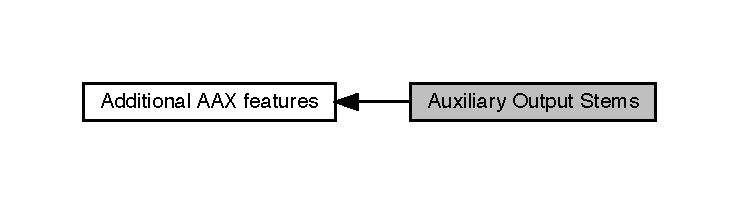
\includegraphics[width=350pt]{a00809}
\end{center}
\end{figure}
